\documentclass[a4paper]{article}

%% Language and font encodings
\usepackage[english]{babel}
\usepackage[utf8x]{inputenc}
\usepackage[T1]{fontenc}
\usepackage{setspace}

%% Sets page size and margins
\usepackage[a4paper,top=3cm,bottom=2cm,left=3cm,right=3cm,marginparwidth=1.75cm]{geometry}

%% Useful packages
\usepackage{graphicx}
\usepackage[export]{adjustbox}
\usepackage{amsmath}
\usepackage{graphicx}
\usepackage[colorinlistoftodos]{todonotes}
\usepackage[colorlinks=true, allcolors=blue]{hyperref}
\usepackage{rotating}
\usepackage{indentfirst}
\usepackage{mathtools}
\DeclarePairedDelimiter\floor{\lfloor}{\rfloor}

\onehalfspacing
\title{Calculating PI using Parallel Processing}
\author{Yiren Wang}

\begin{document}
\maketitle

\newpage
\section{Pre-Processing}
We would like to approximate $\pi$ by calculating this integral: $$\int_0^1 \frac{4}{1 + x^2} \mathrm{d}x$$
\\
In order to approximate an integral, we approximate the area under the function by dividing it into trapezoids. We can divide the segment $[a,b]$ into $n$ sections and calculate the area of the trapezoid for each section. We define the step $h$ as $\frac{a-b}{n}$
\\\\
The area of one trapezoid at the $i^{th}$ position is $$A(i) = \frac{h}{2}[f(a + ih) + f(a + (i+1)h)]$$. 
\\
To approximate $pi$, we'll sum this area from $i=0$ to $i=n$. By writing it out, we can see that we are summing twice $f(a + ih)$ for all $i$ other than $i=0$ and $i=n$. Therefore the total area can be written out as : 
$$ pi \approx \frac{f(b) - f(a)}{2} + \sum_{i=1}^{n-1}A(i)  $$

\section{Processing}
\smallskip
How do we implement this so that it can be calculated in a parallel manner ? 
\\\\
The calculation $A(i)$ for all $i$ is independent, meaning that they can be calculated in any order. We can calculate different chunks of the segment $[0,1]$ on each processor and send the result to the main processor with MPI. Let $p$ be the number of processors. We naturally send an equal load of $\frac{n}{p}$ calculations to each processor. However, it may be that $n$ is not divisible by $p$. We need to ensure that all the calculations are completed, thus the first process will have $\floor{\frac{n}{p}} + n - p\floor{\frac{n}{p}}$ calculations. 

\newpage
\section{Post-Processing}
\subsection{Time}
The following graph shows how much time was necessary to compute the value of pi given the number of subdivisions used. The blue graph indicates the time taken for 4 processes while the orange graph indicates the time taken for 2 processes. While the total time take is generally proportional to the number of trapezoids, it varies quite wildly. Nonetheless we can see that having more processes to share the workload slightly reduces the average time of computation. 
\\\\
\begin{figure}[h]
\caption{Time take to compute $\pi$ given $n$}
\centering
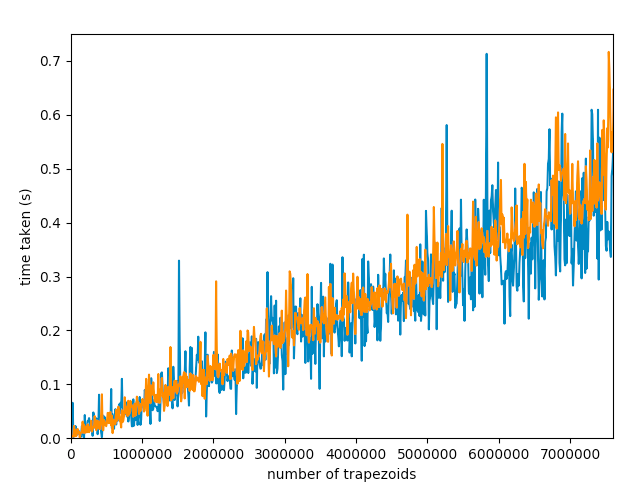
\includegraphics[width=11cm, height=10cm]{time}
\end{figure}

\newpage
\subsection{Accuracy}
As expected, the higher the number of trapezoids used to calculate $\pi$, the better the results are. However, we can see that after $n=100000$, the improvements are no longer significant.  
\\\\

\begin{figure}[h]
\caption{Accuracy of $\pi$ given $n$}
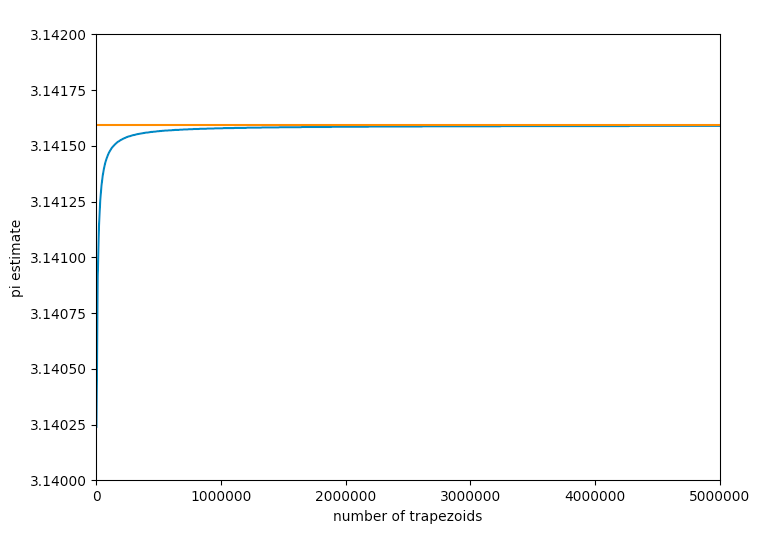
\includegraphics[width=8cm, height=8cm]{pi5mil}
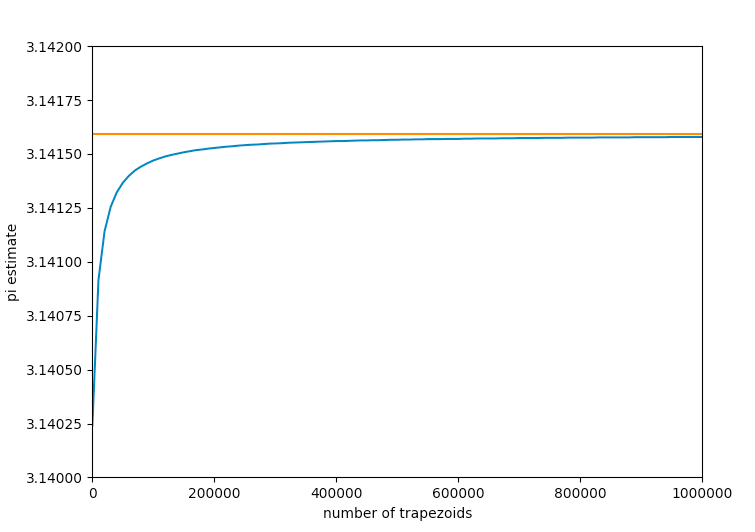
\includegraphics[width=8cm, height=8cm]{pi1mil}
\end{figure}



\end{document}